\vspace{-65pt}
%
\includegraphics[width=1\linewidth]{wobble-2-mosaic-v2-CV}
%\vspace{5pt}

%\cvsection{Career Goals}
%\begin{itemize}
%    \item LLMs \& Natural Language Processing
%    \item Computer vision
%\end{itemize}

\cvsection{Skills}

% ML & AI
\cvskill{MLOps \& Production ML}{4}
\cvskill{LLMs \& RAG Systems}{5}
\cvskill{Computer Vision}{4}
\cvskill{Graph Neural Networks}{4}
\cvskill{Uncertainty Quantification}{4}
\cvskill{Causal Inference}{3}

% Domain Expertise
\cvskill{System Design}{5}
\cvskill{Technical Leadership}{5}
\cvskill{ML for Healthcare}{4}
\cvskill{ML for FinTech}{4}
\cvskill{Geospatial Analytics}{4}
\cvskill{Data Projects Management}{4}

% Infrastructure & Cloud
\cvskill{Azure Cloud Platform}{3}
\cvskill{Databricks \& Big Data}{4}
\cvskill{Docker \& Containerization}{4}
\cvskill{CI/CD Pipelines}{4}

% Programming & Development
\cvskill{SQL \& Database Design}{4}
\cvskill{Julia}{4}
\cvskill{System Programming (C/C++)}{3}

% ML Tools & Frameworks
\cvskill{PyTorch \& Lightning}{5}
\cvskill{Pandas \& Data Engineering}{5}
\cvskill{LangChain Ecosystem}{5}
\cvskill{Vector Databases}{4}
\cvskill{MLflow \& Experiment Tracking}{4}
\cvskill{FastAPI \& API Design}{4}

\cvsection{Proficiency}
\cvskill{Portuguese (native speaker)}{5}
\cvskill{English}{5}
\cvskill{Spanish}{3}

\cvsection{Most Proud of}


\cvachievement{\faTable}{\href{https://link.springer.com/article/10.1007/s00521-019-04144-6}{Gender Bias in Machine Translation}}{Our 2018 research measured the prevalence of male defaults in Machine Translation tools}

\cvachievement{\faHeartbeat}{\href{https://patents.justia.com/inventor/marcelo-de-oliveira-rosa-prates}{VO2 Max for Samsung Galaxy Watch}}{Led the development and global deployment of VO2 max estimation feature, now available to millions of users worldwide}

\cvachievement{\faMap}{\href{https://github.com/marceloprates/prettymaps}{Prettymaps}}{
Python library for drawing pretty maps from OpenStreetMap data (1st place on Hacker News, >11.000 stars, ranked among the 2000 most starred repositories on GitHub)
}
\begin{center}
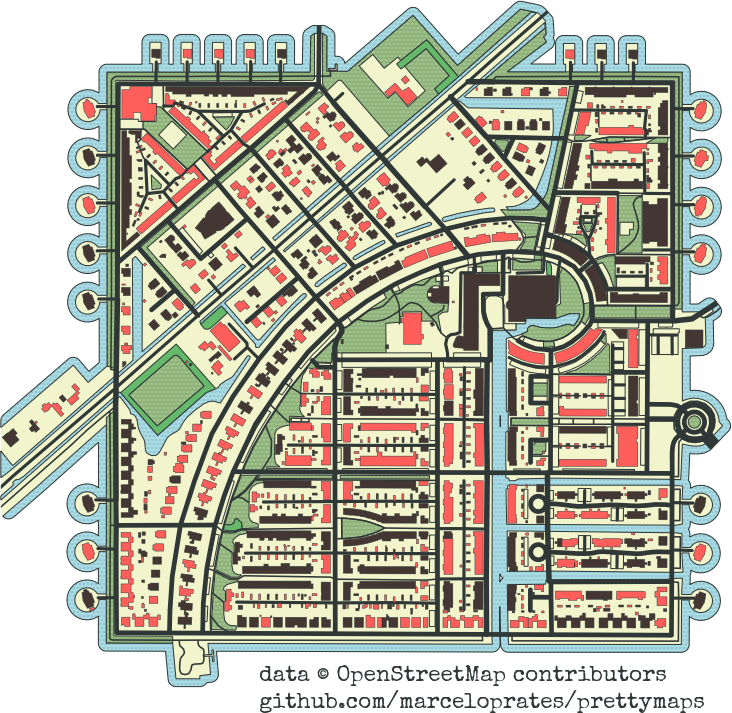
\includegraphics[width=.8\linewidth]{../img/heerhugowaard-CV}
\end{center}
